\documentclass[a4paper]{article}
\usepackage{graphicx,subcaption}
\usepackage{amsmath,amsfonts}
\usepackage{qtree}
\usepackage{tikz}
\title{Notes on Sequence Modelling}
\author{G.A. Jarrad}
\begin{document}
\maketitle
\numberwithin{equation}{section}
\numberwithin{figure}{section}
\numberwithin{table}{section}
\section{Introduction}\label{sec:intro}
blah, blah, blah

\section{Random Process Sequences}
\label{sec:random-processes}
Consider, in general terms, a random process $R$ that generates a sequence of variables,
$R_1,R_2,R_3,\ldots$, where the index $i$ gives the discrete {\em stage} in the sequence,
and each variable $R_i$ randomly takes some value $r_i\in{\cal R}$.
Then, for some arbitrary sequence length $n$, we define
\begin{eqnarray}
\vec{R}_n & = & (R_1,R_2,\ldots,R_n)
\end{eqnarray}
 to be a length-$n$ process sequence, i.e. $|\!\vec{R}_n\!|=n$,
and further define
\begin{eqnarray}
\vec{r}_n & = & (r_1,r_2,\ldots,r_n)\,\in\,{\cal R}^n
\end{eqnarray}
to be a corresponding length-$n$ observation sequence of values.
The probability (for a discrete-value process) or probability density (for a continuous-value process) 
of a given sequence $\vec{r}_n$ is then defined as
\begin{eqnarray}
p(\vec{R}_n=\vec{r}_n)
& = & p(R_1=r_1,\ldots,R_n=r_n)\,.
\end{eqnarray}
Hence, note that if $R$ is a discrete-value process then we must have
\begin{eqnarray}
\hspace*{-5mm}
\sum_{\vec{r}_n\in{\cal R}^n}
p(\vec{R}_n=\vec{r}_n)
& = & \sum_{r_1\in{\cal R}}\cdots\sum_{r_n\in{\cal R}}
p(R_1=r_1,\ldots,R_n=r_n)~~=~1\,.
\end{eqnarray}
Similarly, if $R$ is a continuous-value process, then we must instead have
\begin{eqnarray}
\hspace*{-5mm}
\int_{{\cal R}^n}
p(\vec{R}_n=\vec{r}_n)
\;d\!\vec{r}_n
& \!\!\!=\!\!\! & \int_{\cal R}\!\!\cdots\!\int_{\cal R}
p(R_1=r_1,\ldots,R_n=r_n)\;dr_1\cdots dr_n=1\,.
\end{eqnarray}
In other words, given the sequence length $n$, the set ${\cal R}^n$ of all possible sequences
$\vec{r}_n$ covers the entire probability space.

This summation property causes modelling problems if we do not know in advance the exact length of
a sequence. For example, if the set of all length-1 sequences already
covers the entire probability space, and so too does the set of all length-2 sequences,
then the set of all length-1 and length-2 sequences covers the space twice over.
This problem, however, only exists due to our ambiguous notion of a sequence.
In practice,  suppose we have observed a given sequence 
$\vec{r}_n$. How do we know if the
underlying process $R$ has terminated, or will instead
continue to generate another observed value
$r_{n+1}$, leading to the extended sequence
$\vec{r}_{n+1}$? 
Similarly, how do we know that the first observed value $r_1$ was not in fact
part of a longer, unobserved sequence of values $\ldots,r_{-2},r_{-1},r_0$?

In order to handle such difficulties, we distinguish between a so-called
{\em incomplete} sequence $\vec{R}_n$, and a {\em complete}
sequence $\langle\vec{R}_n\rangle$ that has definite stages of
initiation and termination\footnote{Thus, we see that each length-2 incomplete sequence $\vec{r}_2$ starts with a length-1 incomplete
sequence $\vec{r}_1$, so that measuring the set of all length-1 and length-2 incomplete sequences
amounts to double counting.}.
A complete sequence may be specified by introducing indicator variables
that define the start and end of the sequence.
Thus, indicator $\iota_0$ takes a value of 1 if the sequence
starts at stage 0 (i.e.\ just prior to $R_1$), 
or a value of 0 if it does not.
Similarly, indicator $\tau_{n+1}$ takes a value of 1 if the
sequence terminates at stage $n+1$ (i.e. immediately after $R_n$), or a value of 0 if it does not.
The probability (or probability density)
of a given complete sequence $\langle\vec{r}_n\rangle$ is then defined as
\begin{eqnarray}
p(\langle\vec{r}_n\rangle)
& = & p(\iota_0=1,R_1=r_1\ldots,R_n=r_n,\tau_{n+1}=1)\,.
\end{eqnarray}
The augmented random process is depicted in Figure~\ref{fig:random-process}.
\begin{figure}[hbt]
\centering
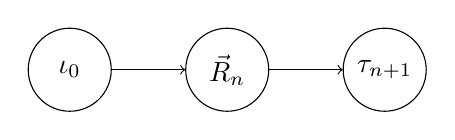
\begin{tikzpicture}[every node/.style={draw,circle,minimum size=3em,inner sep=3pt}]
    \node (1) at (0,0) {$\iota_0$};
    \node (2) at (2, 0)  {$\vec{R}_n$};
    \node (3) at (4, 0) {$\tau_{n+1}$};

    \draw[->] (1) edge (2) ;
    \draw[->] (2) edge (3) ;
\end{tikzpicture}
\caption{A random process for generating both complete and incomplete sequences of length $n$.}
\label{fig:random-process}
\end{figure}

We may also consider {\em partially complete} sequences, namely
the {\em start sequence}
$\langle\vec{R}_n]$, which was initiated at stage 0 but not yet definitely terminated
(i.e.\ $\iota_0=1$ but $\tau_{n+1}$ is unknown),
and the {\em end sequence} $[\vec{R}_n\rangle$, which was terminated at stage $n+1$ but not
definitely initiated at stage 0 (i.e. $\tau_{n+1}=1$ but $\iota_0$ is unknown).
The probability
of a given start sequence $\langle\vec{r}_n]$ is then defined as
\begin{eqnarray}
p(\langle\vec{r}_n]) & = & p(\iota_0=1,R_1=r_1\ldots,R_n=r_n)\,,
\end{eqnarray}
and the probability of the end sequence $[\vec{r}_n\rangle$ is
\begin{eqnarray}
p([\vec{r}_n\rangle)
& = & p(R_1=r_1\ldots,R_n=r_n,\tau_{n+1}=1)
\end{eqnarray}
for an end sequence.
In the special case where we know in advance that a start sequence definitely does not terminate
at stage $n+1$ (i.e.\ $\tau_{n+1}=0$),  we may instead write
\begin{eqnarray}
p(\langle\vec{r}_n!)
& = & p(\iota_0=1,R_1=r_1\ldots,R_n=r_n,\tau_{n+1}=0)\,.
\end{eqnarray}
Likewise, if an end sequence definitely does not initiate at stage
0 (i.e.\ $\iota_0=0$), then
\begin{eqnarray}
p(!\vec{r}_n\rangle)
& = & p(\iota_0=0,R_1=r_1\ldots,R_n=r_n,\tau_{n+1}=1)\,.
\end{eqnarray}

Hence, for a discrete-value process, the probability mass of all complete length-$n$ sequences is given by
\begin{eqnarray}
\hspace*{-5mm}
\sum_{\vec{r}_n\in{\cal R}^n}
p(\langle\vec{r}_n\rangle)
& = & p(\iota_0=1,\tau_{n+1}=1)
~\doteq~P(N=n)\,,
\end{eqnarray}
where we have introduced the random variable $N$ to denote the length of an
arbitrary complete sequence. 
%Similarly,
%\begin{eqnarray}
%\hspace*{-5mm}
%\sum_{\vec{r}_n\in{\cal R}^n}
%p(\langle\vec{r}_n!)
%& = & p(\iota_0=1,\tau_{n+1}=0)
%~\doteq~P(N>n)\,,
%\end{eqnarray}
For the corresponding continuous-value process, we likewise deduce that
\begin{eqnarray}
%\hspace*{-5mm}
\int_{{\cal R}^n}
p(\langle\vec{r}_n\rangle)\;d\!\vec{r}_n
& = & 
p(\iota_0=1,\tau_{n+1}=1)
~=~P(N=n)\,.
\end{eqnarray}
We therefore deduce that the set ${\cal R}^{*}=\bigcup_{n=0}^{\infty}{\cal R}^n$ 
of all complete sequences of arbitrary length
covers the entire probability space exactly once, since for the discrete-value case we have
\begin{eqnarray}
\sum_{\vec{r}_{*}\in{\cal R}^{*}}
p(\langle\vec{r}_{*}\rangle)
& = & \sum_{n=0}^{\infty}
\sum_{\vec{r}_n\in{\cal R}^n}
p(\langle\vec{r}_n\rangle)
~=~\sum_{n=0}^{\infty}P(N=n)~=~1\,,
\end{eqnarray}
and for the continuous-value case we have
\begin{eqnarray}
\int_{{\cal R}^{*}}
p(\langle\vec{r}_{*}\rangle)
\;d\!\vec{r}_{*}
& = & \sum_{n=0}^{\infty}
\int_{{\cal R}^n}
p(\langle\vec{r}_n\rangle)
\;d\!\vec{r}_n
~=~\sum_{n=0}^{\infty}P(N=n)~=~1\,.
\end{eqnarray}

%%%%%%%%%%%%%%%%%%%%%%%%%%%%%%%%%%%
\section{Markov Process Sequences}
\label{sec:markov-processes}
In Section~\ref{sec:random-processes} we defined random processes and the sequences they generate.
We now assume that the random process $R$ is also {\em causal}, meaning that the distribution of
values for variable $R_t$, at stage $t$, depends entirely upon the values generated previously
in the sequence at stages $t-1,t-2,\ldots,1$. In addition, for a complete sequence
the distribution of the variable $R_1$ at the initial stage depends strongly upon being first
in the sequence, and likewise the distribution of the variable $R_n$, for a length-$n$
sequence, depends strongly upon the past values in the sequence and weakly on the fact
that it is the final stage.
Hence, the probability of a complete, causal sequence is taken here to be
\begin{eqnarray}
p(\langle\vec{r}_{n}\rangle)
& = & 
p(\iota_0=1)\;
\prod_{t=1}^{n}
p(R_t=r_t\;|\;\vec{R}_{t-1}=\vec{r}_{t-1},\iota_0=1)
\nonumber\\&&
p(\tau_{n+1}=1\;|\;\vec{R}_{n}=\vec{r}_{n},\iota_0=1)
\,.
\label{eq:temporal-model}
\end{eqnarray}
The causal process is depicted in Figure~\ref{fig:causal-process}.
\begin{figure}[hbt]
\centering
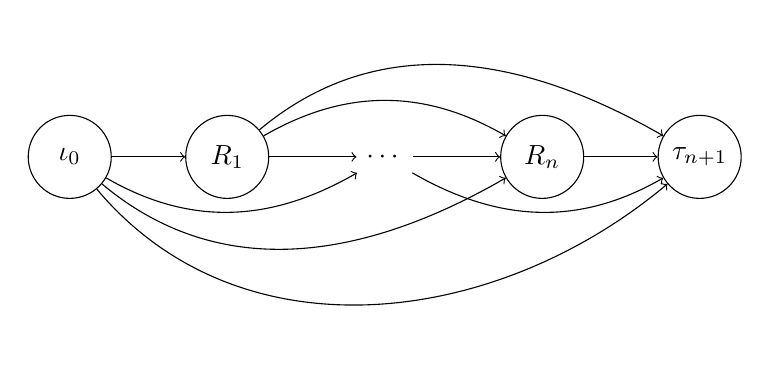
\begin{tikzpicture}[cnode/.style={draw,circle,minimum size=3em,inner sep=3pt}]
    \node[cnode] (0) at (0,0) {$\iota_0$};
    \node[cnode] (1) at (2,0) {$R_1$};
    \node (any) at (4,0) {$\cdots$};
    \node[cnode] (n) at (6, 0)  {$R_n$};
    \node[cnode] (np1) at (8, 0) {$\tau_{n+1}$};

    \draw[->] (0) edge (1) ;
    \draw[->] (0) to[out=-30,in=-150] (any) ;
    \draw[->] (0) to[out=-40,in=-150] (n) ;
    \draw[->] (0) to[out=-50,in=-140] (np1) ;

    \draw[->] (1) edge (any) ;
    \draw[->] (1) to[out=30,in=150] (n) ;
    \draw[->] (1) to[out=40,in=150] (np1) ;

    \draw[->] (any) edge (n) ;
    \draw[->] (any) to[out=-30,in=-150] (np1) ;

    \draw[->] (n) edge (np1) ;
\end{tikzpicture}
\caption{A fully-connected causal process for generating temporal sequences of length $n$.}
\label{fig:causal-process}
\end{figure}

The related models for partially complete or incomplete sequences may be similarly obtained
by suitably modifying the corresponding boundary conditions for $\iota_0$ and $\tau_{n+1}$
--- refer to Section~\ref{sec:random-processes}.
In general, all types of sequences may be handled by a slight change of notation.
Let $V$ denote an arbitrary node variable, such that $V_0=\iota_0$, $V_t=R_t$ for $t=1,2,\ldots,n$,
and $V_{n+1}=\tau_{n+1}$, and consider $\vec{V}=(V_0,\ldots,V_{n+1})$. 
Likewise, let $\vec{v}$ denoted an observed sequence of values, e.g.\ $\vec{v}=\langle\vec{r}_n\rangle$, or
$\vec{v}=[\vec{r}_n\rangle$, et cetera. Then the causal process model~\eqref{eq:temporal-model} reduces to
\begin{eqnarray}
p(\vec{v}) & = & \prod_{t=0}^{n+1}p(V_t=v_t\;|\;\vec{\Pi}_t(\vec{V})=\vec{\pi}_t(\vec{v}))\,,
\end{eqnarray}
where $\vec{\Pi}_t(\vec{V})=(V_0,V_1,\ldots,V_{t-1})$ denotes the predecessor nodes upon which node $V_t$
is conditionally dependent, and 
$\vec{\pi}_t(\vec{v})=(v_0,v_1,\ldots,v_{t-1})$ similarly denotes the observed values of those predecessor nodes. 

In practice, the causal model is usually simplified further by limiting the 
conditional dependency on past values to a maximum number $m$ of terms.
Hence, this so-called {\em $m$-th order Markov model} is given by
\begin{eqnarray}
p(\vec{v}) & = & \prod_{t=0}^{n+1}p(V_t=v_t\;|\;\vec{\Pi}^{(m)}_t(\vec{V})=\vec{\pi}_t^{(m)}(\vec{v}))\,,
\end{eqnarray}
where the predecessor nodes are now given by
\begin{eqnarray}
\vec{\Pi}_t^{(m)}(\vec{V}) & = & 
\left\{
\begin{array}{ll}
(V_0,V_1,\ldots,V_{t-1}) & \mbox{if }t\le m\,,
\\
(V_{t-m},V_{t-m+1},\ldots,V_{t-1}) & \mbox{if }t>m
\end{array}
\right.\,.
\end{eqnarray}
An example from the realm of natural language understanding is the lexicographical analysis of the character
sequences of words using bigrams (pairs of adjacent characters, corresponding to $m=1$), and trigrams 
(triples of adjacent characters, corresponding to $m=2$), et cetera.

In the special case of $m=1$, the first-order Markov model takes on the even simpler form
\begin{eqnarray}
p(\vec{v}) & = & \prod_{t=0}^{n+1}p(V_t=v_t\;|\;V_{t-1}=v_{t-1})\,.
\end{eqnarray}
This process is depicted in Figure~\ref{fig:markov-1-process}.
\begin{figure}[hbt]
\centering
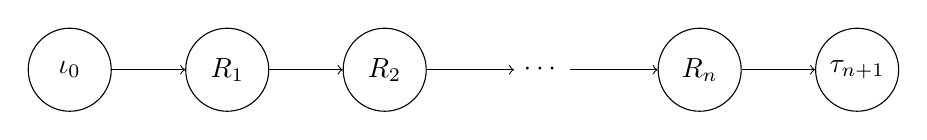
\begin{tikzpicture}[cnode/.style={draw,circle,minimum size=3em,inner sep=3pt}]
    \node[cnode] (0) at (0,0) {$\iota_0$};
    \node[cnode] (1) at (2,0) {$R_1$};
    \node[cnode] (2) at (4,0) {$R_2$};
    \node (any) at (6,0) {$\cdots$};
    \node[cnode] (n) at (8, 0)  {$R_n$};
    \node[cnode] (np1) at (10, 0) {$\tau_{n+1}$};

    \draw[->] (0) edge (1) ;
    \draw[->] (1) edge (2) ;
    \draw[->] (2) edge (any) ;
    \draw[->] (any) edge (n) ;
    \draw[->] (n) edge (np1) ;
\end{tikzpicture}
\caption{A first-order Markov process for generating causal sequences of length $n$.}
\label{fig:markov-1-process}
\end{figure}

%%%%%%%%%%%%%%%%%%%%%%%%%%%%%%%%%%%%
\end{document}
